\documentclass[11pt,a4paper]{report}
\usepackage[utf8]{inputenc}
\usepackage{amsmath}
\usepackage{amsfonts}
\usepackage{amssymb}
\usepackage{graphicx}
\usepackage{pgfplots}
\usepackage{circuitikz}
\usepackage{hyperref}
\usepackage{tikz}
\usepackage{pdfpages}
\usepackage{minted}
\usepackage{mathtools}
	\definecolor{bg}{rgb}{0.95,0.95,0.95}
\usetikzlibrary{calc,trees,positioning,arrows,chains,shapes.geometric,%
	decorations.pathreplacing,decorations.pathmorphing,shapes,%
	matrix,shapes.symbols}

\tikzset{
	>=stealth',
	punktchain/.style={
		rectangle, 
		rounded corners, 
		draw=black, very thick,
		text width=10em, 
		minimum height=3em, 
		text centered, 
		on chain},
	line/.style={draw, thick, <-},
	element/.style={
		tape,
		top color=white,
		bottom color=blue!50!black!60!,
		minimum width=8em,
		draw=blue!40!black!90, very thick,
		text width=10em, 
		minimum height=3.5em, 
		text centered, 
		on chain},
	every join/.style={->, thick,shorten >=1pt},
	decoration={brace},
	tuborg/.style={decorate},
	tubnode/.style={midway, right=2pt},
}

\pgfmathdeclarefunction{gauss}{2}{%
	\pgfmathparse{1/(#2*sqrt(2*pi))*exp(-((x-#1)^2)/(2*#2^2))}%
}

\title{Relatório 1  \\
	Projeto em Eletrônica I - EEL7801 \\ \vfill
	\normalsize{Universidade Federal de Santa Catarina - UFSC \\
		Professora: Daniela Ota Hisayasu Suzuki}
	\author{
		{Luiz Augusto Frazatto Fernandes: \it{17202752}} \\
		{Leonardo José Held: \it{17203984}}
	}
}
\date{02 de Maio de 2019}
\begin{document}
	

	\maketitle
	%todo: atualizar pro link do github do Robota quando empurrarmos o projeto pra lá
		\newpage Nota: O projeto todo, incluindo este documento e os demais códigos de simulação e de projeto podem ser encontrados em \url{https://github.com/leonheld/EEL7801}
	\\
	
	Nota de Trademark: \\
	
	Arm™, ARM™, Cortex™ são marcas registradas da Arm Limited.
	Copyright © 1995-2019 Arm Limited (or its affiliates).\\
	
	STM32CubeMX™, ST™, ST-Link™ são marcas registradas da Singapore Technologies Engineering Limited.
	Copyright © 2019 Singapore Technologies Engineering Ltd.\\
	
	GCC is Copyright (C) 1986, 1987, 1988, 1989, 1990, 1991, 1992, 1993, 1994,
	1995, 1996, 1997, 1998, 1999, 2000, 2001, 2002, 2003, 2004, 2005, 2006, 2007,
	2008 Free Software Foundation, Inc.
	
	Octave is Copyright © 1996-2016 John W. Eaton. 
	
	\setcounter{chapter}{0}
	\chapter{Metodologia}
	\section{Modulação e demodulação de sinais}
	\subsection{Motivação da escolha do algoritmo}
	
	Escolheu-se o processo de modulação por Chaveamento de Deslocamento de Frequência (FSK, em inglês). São usadas duas frequências ótimas para se representar 0 e 1, e ambas são obtidas experimentalmente: a partir de testes realizados com o transdutor (microfone), é gerada uma curva normal, em que a resposta desse ao sinal recebido é ótima para uma frequência específica (frequência da onda portadora). São, então, obtidas duas outras frequências equidistantes do centro da curva gaussiana, e a cada uma é associado um valor binário.
	
	
	O processo de modulação, em si, consiste na transformação de um sinal PWM em um analógico (que é controlado por um STM32) que, por sua vez, é emitido por um tweeter. O sinal (sonoro) é recebido por um microfone controlado por outro STM32, que realizará o processo de demodulação do sinal.
	\subsection{Algoritmo da modulação (FSK)}	

	Empiricamente são testadas (com o microfone) diferentes frequências emitidas pelo tweeter e recebidas pelo microfone. A de melhor resposta (dada, no gráfico abaixo, por $f$) é associada à onda portadora (carrier). É, então, estabelecido um desvio $\Delta{f}$, e, a partir desse, são determinadas:
	\begin{center}
		\begin{align*}
		f_L = f - \Delta{f}\\
		f_H = f + \Delta{f}
		\end{align*}
	\end{center}
	de tal forma que à $f_H$ se associa o bit $1$, e à $f_L$, $0$.
	

	
	\begin{center}
		\begin{tikzpicture}
		\begin{axis}[every axis plot 
		post/.append style={
		mark=none,domain=0:50, samples=50,smooth},
		axis x line*=bottom,
		axis y line*=left,
		xlabel = {Frequência},
		ylabel = {Resposta (queda de tensão/potência)},
		xtick=\empty,
		ytick=\empty,	
		enlargelimits=upper]
		\addplot[mark=*] coordinates {(25,10^-1)} node[pin=270:{$f$}]{} ;
		\addplot[mark=*] coordinates {(23,8*10^-2)} node[pin=150:{$f_L$}]{} ;
		\addplot[mark=*] coordinates {(27,8*10^-2)} node[pin=30:{$f_H$}]{} ;
		\addplot{gauss(25,4)};
		\end{axis}
		\end{tikzpicture}
	\end{center}


Há, também, uma segunda possibilidade: de o microfone não reagir significativamente a diferentes frequências, mas de ainda assim conseguir diferenciá-las. Isto é: o microfone identifica quando duas frequências recebidas são diferentes, mas sua curva de queda de tensão se aproxima de uma constante, como no exemplo a seguir:


\begin{center}
	\begin{tikzpicture}
	\begin{axis}[every axis plot 
	post/.append style={
	mark=none,domain=6:50, samples=50,smooth},
	axis x line*=bottom,
	axis y line*=left,
	xlabel = {Frequência},
	ylabel = {Resposta (queda de tensão/potência)},
	xtick=\empty,
	ytick=\empty,	
	enlargelimits=upper]
	\addplot {2}; 
	\end{axis}
	\end{tikzpicture}
\end{center}


	Caso esse comportamento seja verificado, o que há de se fazer é, simplesmente, escolher duas frequências quaisquer para se trabalhar no algoritmo.

\subsection{Obtenção das frequências ótimas}
\paragraph{}
Por meio do circuito abaixo é medida a tensão/potência dissipada nos terminais do microfone. A curva (próxima à normal descrita acima) é gerada a partir da potência consumida/queda de tensão que é medida entre os terminais do microfone.


\begin{center}
	\begin{circuitikz} \draw
		(0,0) to (6,0) 
		to [vR, l=$Microfone$] (6,3)
		to [resistor, l=$R$] (0,3)
		to [vsourcesin, l= $Gerador$] (0,0)
		(2,0) to (2,-1) node[ground] {}
		(6,0) -- (9,0)
		(6,3) to (9,3)
		(9,0) to [voltmeter, l=$Voltimetro$] (9,3)
		;
	\end{circuitikz}
\end{center}


Quanto maior a queda de tensão no microfone, maior a energia por ele consumida em relação ao resto do circuito (divisor de tensão), logo, melhor será sua resposta aos estí­mulos sonoros testados.

	\subsection{Tratamento do sinal analógico}

Será utilizado, a priori, um filtro passa-baixa a fim de reduzir o ruído de alta frequência, além de um amplificador não inversor (que garantirá uma clara análise do sinal).

\begin{center}
	\begin{circuitikz} \draw
		(0, 0) node[op amp, yscale=-1] (opamp) {}
		(opamp.+) -- (-3, 0.5)
		to[C, l=$C$] (-3, -4)
		(-3, 0.5) to[R, *-, l=$R_1$] (-6, 0.5) node[label={$V_{in}$}] {}
		(opamp.-) to[short,*-] ++(0,-1.5) coordinate (leftR)
		to[R, l=$R_3$] (leftR -| opamp.out)
		to[short,-*] (opamp.out)
		to ++(1,0) node[label={$V_{out}$}] {}
		(-1, -2) to[R, *-, l=$R_2$] (-1,-4)
		(-3, -4) -- (-1, -4)
		(-2,-4) to (-2,-5) node[ground] {}
		;
	\end{circuitikz}
\end{center}


	A frequência de corte do circuito acima é dada por \newline
	\begin{equation}
	f_c = \frac{1}{2\cdot\pi\cdot{R_1}\cdot{C}}
	\end{equation}
	
	
	E o ganho por \newline
	\begin{equation}
	\frac{V_{out}}{V_{in}} = G = 1 + \frac{R_3}{R_2}
	\end{equation}
	
	
	Espera-se trabalhar com frequências na faixa audível ($20 Hz$ a $20 kHz$). Portanto, pode-se colocar uma frequência de corte razoável de 22 kHz a priori, já que, dessa forma, o ruído de alta frequência filtrado não interferirá nos sinais desejados.
	
	
	Para tal, usamos um capacitor com capacitância $C = 0.1\mu{F}$, o que nos resulta:
	
	\begin{equation}
	R_1 = \frac{1}{2\cdot{\pi}\cdot{0.1}\cdot{10^{-6}}\cdot{22}\cdot{10^3}} \approx 72\Omega 
	\end{equation}
	
	Para avaliarmos o ganho, deixamos em $R_3$ um potenciômetro e, assim, avaliamos, a posteriori, qual o melhor ganho para se projetar (aquele cuja análise posterior for facilitada).


		\subsection{Circuito amplificador}
	\paragraph{}
	O núcleo do amplificador será o chip {\it LM386}, cuja pinagem pode ser vista abaixo:
		
	\begin{center}
		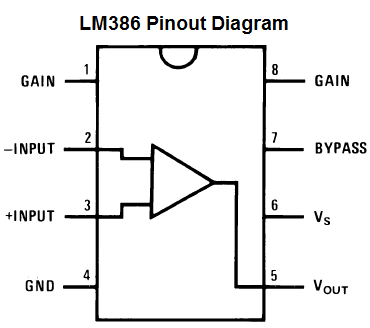
\includegraphics[width=0.5\textwidth]{LM386_pinout_diagram.png}\\
		\footnotesize{Diagrama com pinagem do LM386}
	\end{center}
	
	O circuito abaixo será utilizado a fim de se amplificar o sinal emitido pelo modulador, para que esse seja reproduzido pelo transdutor utilizado.\footnote{http://www.circuitbasics.com/build-a-great-sounding-audio-amplifier-with-bass-boost-from-the-lm386/}\\
	
	\begin{center}
		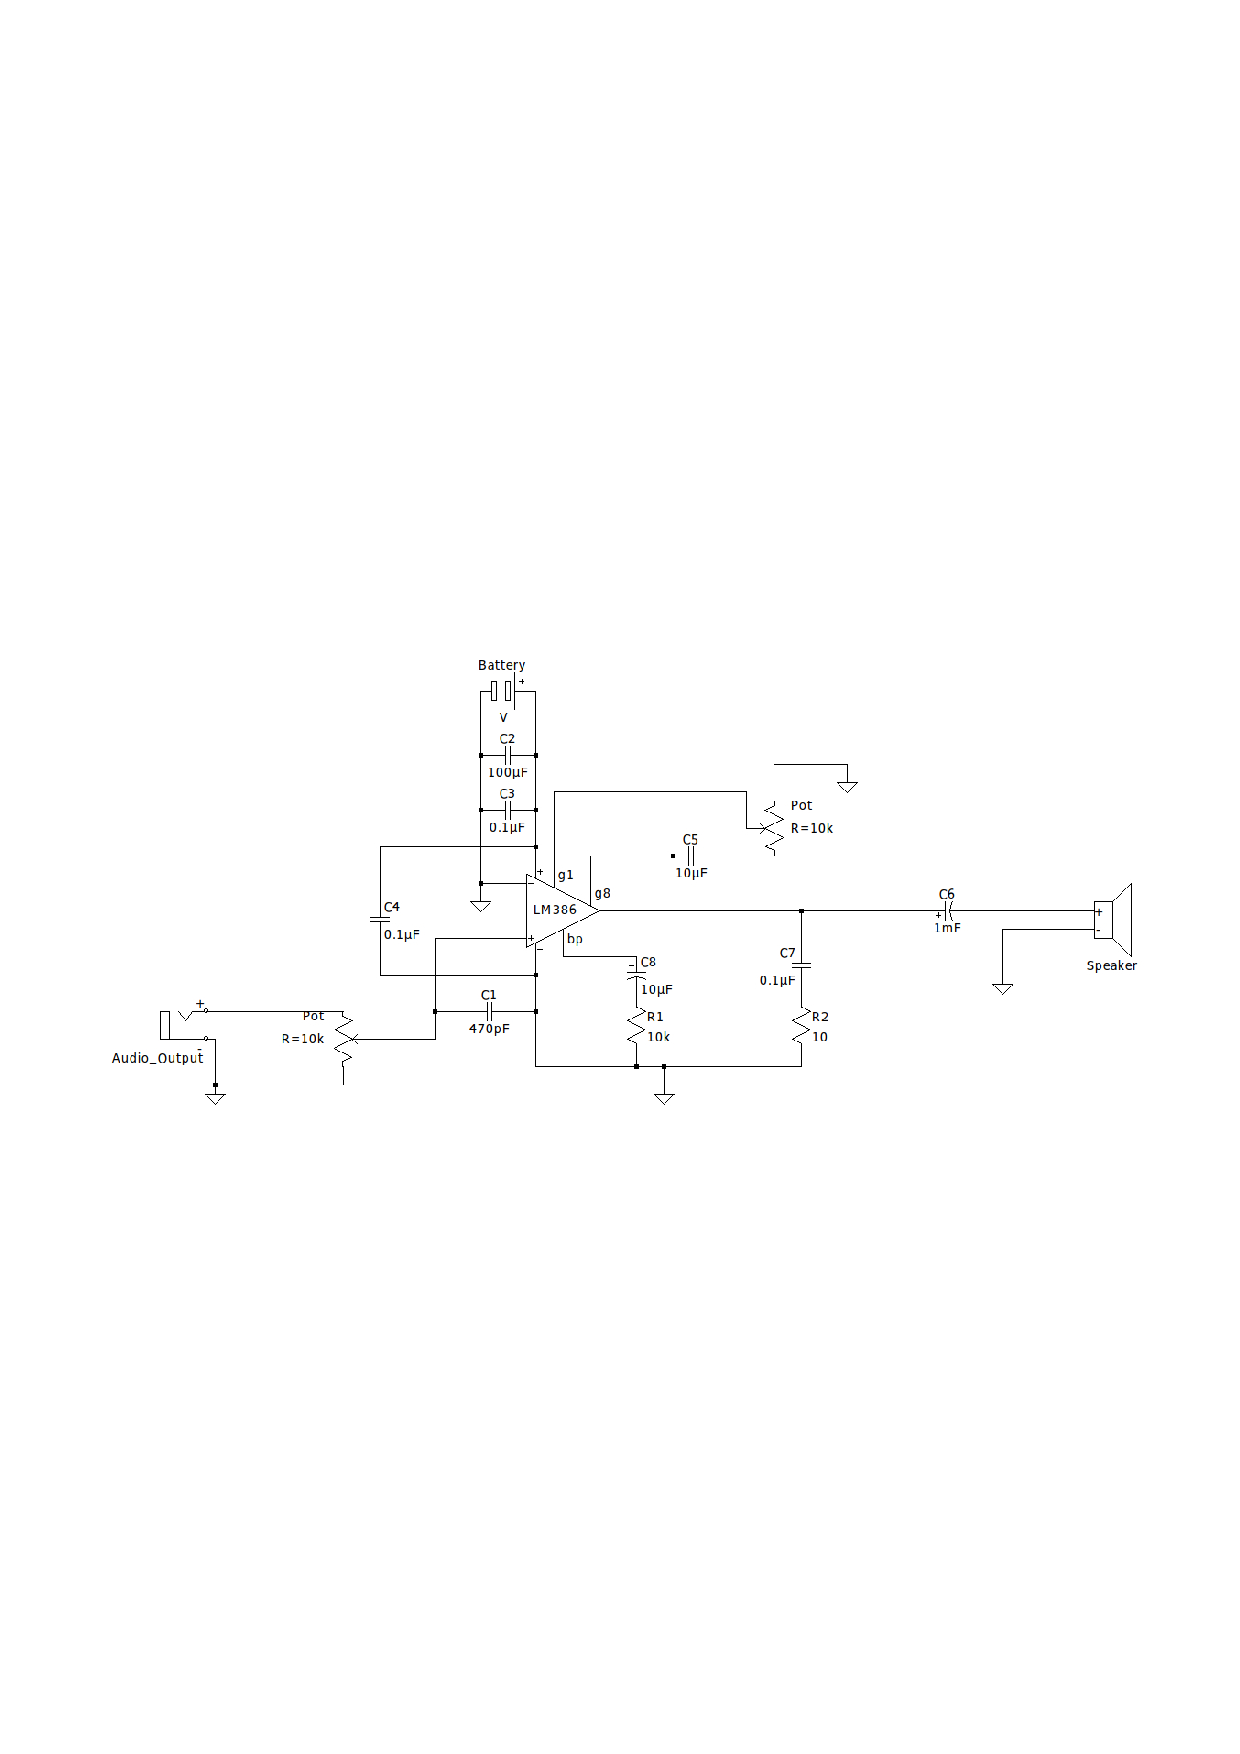
\includegraphics[width=\linewidth]{amplifier_circuit.png}\\
		\footnotesize{Circuito amplificador (conectado entre saída do emissor e entrada do speaker/transdutor)}
	\end{center}}

	\begin{itemize}
		\item[{\bf 1.}]$C_1$ é responsável por filtrar eventuais interferências captadas pelos fios.
		\item[{\bf 2.}]$C_2$ e $C_3$ são responsáveis por desacoplar a fonte do amplificador. o de $100\mu{F}$ filtrará ruído de alta frequência, enquanto o de $0.1\mu{F}$, de baixa.
		\item[{\bf 3.}]$C_4$ desacopla os pinos de alimentação do chip.
		\item[{\bf 4.}]$C_5$, juntamente com o potenciômetro, tem a função de regular o ganho do {\it LM386} entre 20 e 200 vezes.\footnote{http://www.ti.com/lit/ds/symlink/lm386.pdf}
		\item[{\bf 5.}]$C_6$ rejeita correntes contínuas.
		\item[{\bf 6.}]$C_7$ e $R_2$ atuam como um passa-alta, a fim de evitar ruídos no som emitido pelo speaker.
		\item[{\bf 7.}]$C_8$ e $R_1$ desacoplam a entrada de áudio (bypass pin).
		\item[{\bf 8.}]Os potenciômetros têm finalidade de teste (possivelmente serão substituídos por resistores, uma vez devidamente testadas resistências condizentes com o circuito).
	\end{itemize}

\section{Escolha de Microcontrolador ($\mu$C)}
	\subsection{STM32}
	O microcontrolador foi escolhido na base da seguinte {\it criteria}:
	
	\begin{itemize}
		\item[{\bf 1.}]Baixo Custo: O controlador deve ter um custo mínimo, com alta flexibilidade de prototipação. Deve incluir um programador integrado, ou possuir algum de baixo custo e facilmente acessível.
		
		\item[{\bf 2.}] Alto suporte: O controlador deve ter suporte de compiladores, ambientes de programação, comunidade de software aberto e pela própria empresa que o fabrica.
		
		\item[{\bf 3.}] Performance: A unidade deve ter uma performance que faz processamento de dados e sinais com relativa rapidez, de forma que a sua capacidade de processamento não dite o algoritmo e execução do programa.
	
	\end{itemize}

	Em consideração aos items {\bf 1} e {\bf 2}, optou-se por utilizar algum controlador da família ARM™, indubitavelmente a família de processadores mais utilizada no mundo, e desta forma, acessível e de bom suporte. \\
	
	O quesito performance nos faz olhar para as famílias de processadores que a ARM atualmente oferece, dentre as quais, os processadores Cortex-M3 \footnote{https://developer.arm.com/ip-products/processors/cortex-m/cortex-m3} parecem entrar nos quesitos. \\
	
	De acordo com o página da empresa sobre o processador:\\
	
	``The Arm Cortex-M3 processor is the industry-leading 32-bit processor for highly deterministic real-time applications."\\
	
	Depois de uma curta pesquisa de mercado, a placa STM32F103C8 da ST, também conhecida como {\it bluepill}, parece preencher bem os quesitos supraescritos, com um processador Cortex-M3 de 72MHz de clock interno, é um dos microcontroladores mais potentes da categoria fabricados pela ST, o que preenche bem o requisito {\bf 3}.\\
	\begin{center}
		\includegraphics[width=0.5\textwidth]{bluepill}\\
		\footnotesize{STM32F103C8.}
	\end{center}

	
	Qualquer processador dessa linha da ST pode ser programado e debuggado via uma interface chamada ST-Link, que também foi de fácil obtenção e baixo custo, e basicamente inclui um outro processador que conversa em tempo real com a placa alvo.
	\begin{center}
	\includegraphics[width=0.2\textwidth]{stlink}\\
	\footnotesize{Programador SWD ST-Link.}
	\end{center}
	
	\subsection{Suporte}
	O suporte oferecido tanto pela ARM quanto pela ST é extenso. A ST produz seu próprio software de pré-configuração e geração de código chamado STM32CubeMX, que é uma {\it Graphical User Interface} usada para gerar o código inicial, como configuração de clock interno e dos pinos do processador, por exemplo.\\
	
	A ARM também mantém um compilador, um debugger e utilidades de programação para sua linha de processadores, todas as ferramentas baseadas no GCC, GDB e Gnu Binutils.\footnote{https://developer.arm.com/tools-and-software/open-source-software/developer-tools/gnu-toolchain}\\
	
	Como software de upload de código e debugging, podemos usar o programa {\it openocd} \footnote{http://openocd.org/}, também de código aberto que acessa a interface SWD ({\it Serial Wire Debug}) do ST-Link via terminal, com possibilidade de abrir uma janela de sessão de debugging via GDB.
	
	\subsection{Processo de Desenvolvimento}
	Desde a última versão, o STM32CubeMX consegue produzir um Makefile que pode ser compilado pelo programa {\it make} chamando o compilador de C cedido pela ARM.\\
	
	A partir disso, o compilador gera arquivos .hex, .elf e .bin, podendo esses ser inseridos na memória interna do microcontrolador pelo openocd.\\
	
	Para a programação, existe uma HAL - {\it Hardware Abstration Layer} -, também fornecida pela ST, que é incluída nos sources do projeto no momento da inicialização do código pelo STM32CubeMX e possuí funções específicas de baixo nível, mas tem as mesmas chamadas em quaisquer processador alvo que queira executar o código, aumentando a portabilidade. Também, a HAL é construída de forma a aumentar o nível de abstração, diminuindo significativamente a complexidade do código, permitindo desenvolvimento rápido e colaborativo, sem necessariamente conhecer todos os artifícios de baixo nível de cada processador.
	\begin{center}
		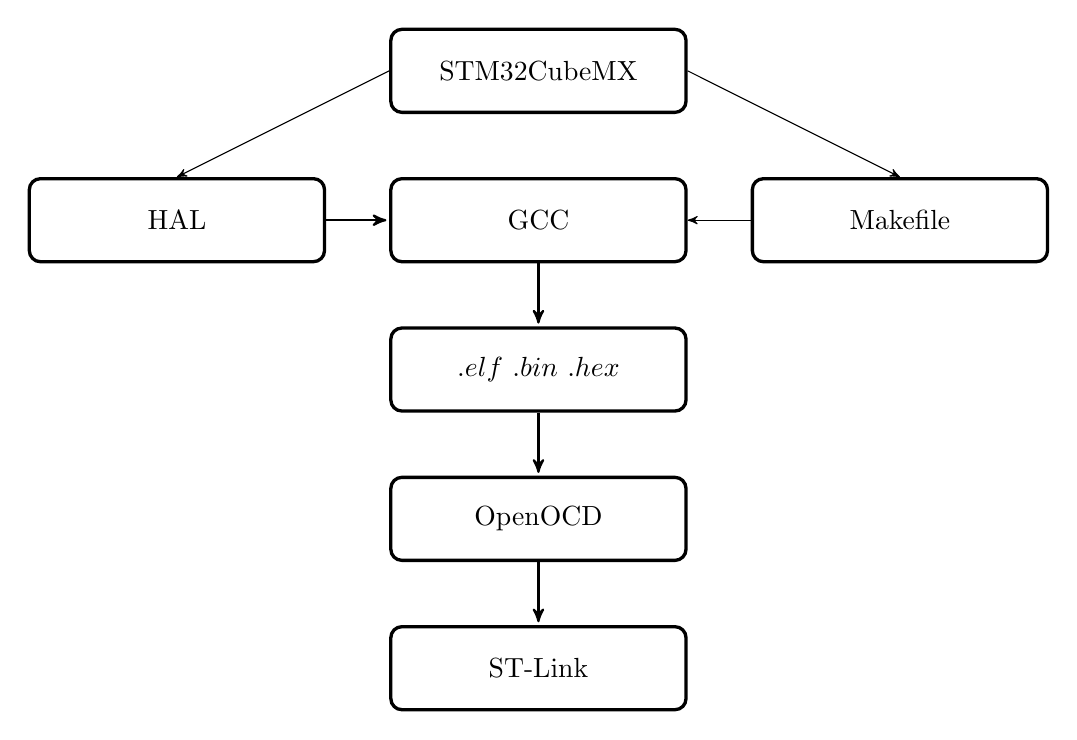
\begin{tikzpicture}
	[node distance=.8cm,
	start chain=going below,]
	
	\node[punktchain, join, ] (STM) {STM32CubeMX};
	\node (gcc) [punktchain ] {GCC};
	\begin{scope}[start branch=top,
	every join/.style={->, thick, shorten <=1pt}, ]
	\node[punktchain, on chain=going left, join=by {<-}](HAL) {HAL};
	\end{scope}
	\begin{scope}[start branch=bottom,]
	\node (makefile) [punktchain, on chain=going right] {Makefile};
	\end{scope}
	\node[punktchain, join,] {$.elf\ .bin\ .hex$};
	\node[punktchain, join,] {OpenOCD};
	\node[punktchain, join]  {ST-Link};
	
	\draw[<-] (gcc.east) -- (makefile.west);
	\draw[<-] (makefile.north) -- (STM.east);
	\draw[<-] (HAL.north) -- (STM.west);
	\end{tikzpicture}\vspace{0.1cm}
	\footnotesize{Flowchart de programação e desenvolvimento do firmware.}
	\end{center}

\chapter{Simulação e Algoritmo}
	\section{Simulação usando Octave}
	
	Os algoritmos foram programandos usando Octave, uma linguagem de manipulação de vetores que possuí pacotes específicos para comunicação e sinais digitais. Também possuí uma função \texttt{agwn}, ou {\it Additive Gaussian White Noise}, que introduz barulho no sistema e no sinal.\\
	
	O algoritmo base de simulação foi pego do site da MathWorks, criadora do MATLAB, linguagem compatível com Octave.  Dessa base, alteramos o código de forma a cortar excessos e tentando eliminar elementos de aleatoriedade, vistos que são mais difíceis de se obter na plataforma de hardware que pretendemos usar. Também modularizamos o código de forma que podemos fazer $n$ simulações com padrões diferentes de onda, {\it sampling rates}, diferentes frequências e tudo entre o meio.\\
	
	O algoritmo é extremamente bem conhecido e documentado. O algoritmo de modulação compreende em gerar uma onda sinusóide que é modulada em função de um vetor binário. De forma resumida:
	\begin{equation}
	\mathfrak{F}(V)\ onde\ V(i) = 1 \lor 0\ para\ i \in \mathbb{N}
	\end{equation}
	e

	\[
	\begin{dcases}
	\mathfrak{F} \coloneqq \delta_{+} & V(i) = 0 \\
	\mathfrak{F} \coloneqq \delta_{-} & V(i) = 1 \\
	\end{dcases}
	\]


	Defina $\mathcal{L}$ como um vetor que receberá um sinal senoidal, dependendo de um fator $\delta_{+/-}$ da função $\mathfrak{F}$

	\begin{equation}
	\mathcal{L} = \mathfrak{F}(V) = \sin{2 \cdot \pi \cdot t \cdot f_{\delta_{+/-}}}
	\end{equation}
	
	Vale reiterar que essa $f$ é baseada numa frequência da onda {\it carrier}. Como estamos destacando frequências diferentes diferentes para cada sinal, a "carrier" é só uma alegoria para determinar frequência e período de uma onda fundamental que nunca será gerada. A alternativa seria usar uma onda continua onde o bit $1$ ou $0$ são gerados a partir de apenas um {\it shift} de frequência, e não dois como estamos fazendo aqui.\\
	
	Dessa forma, se constrói uma onda que varia no tempo e é construída com duas frequências de acordo com os bits do vetor que se deseja modular.\\
	
	Em termos de implementação, é possível direcionar os valores amostrados dessa senóide para um Conversor Digital Analógico, e obter amplificação das mesmas.\\
	
	O resultado da simulação pode ser visto da próxima página. O primeiro gráfico representa uma onda pura, não modulada, a "carrier", que como mencionamos, nunca será gerada no contexto do nosso algoritmo.\\
	
	O segundo gráfico está associado com um pulso quadrado de mensagens que representa o vetor 
	
	\[V = [1 0 1 0 1 1 1 0 0 1]\]
	
	O terceiro gráfico é a onda já modulada, passada pelo algoritmo citado acima. Perceba os cortes horizontais de frequência gerados pelo vetor do pulso quadrado.\\
	
	A quarta onda é a terceira com {\it white noise} adicionado. Podemos usar o white noise como barulho e interferência criado pelo ambiente durante a execução do programa. A razão $\frac{sinal}{noise}$ naquele caso está extremamente alta, da ordem de 100. É perceptível a diferença na onda.
	\includepdf[page={1}]{sinais}
	
	\includepdf[page={1}]{sinais_comp}
	\subsection{demod}
	
	\begin{minted}[frame=lines,
	framesep=2mm,
	baselinestretch=1.2,
	bgcolor=bg,
	fontsize=\footnotesize,
	linenos
	]{matlab}
function [NORMALIZED_BIT_ERROR_RATE] = fsk_demod(sinal_modulado, ruido)

    onda_transmitida = awgn(sinal_modulado, ruido); %adiciona ruido no sinal

    data = [1 0 1 0 1 1 1 0 0 1]; %apenas necessario pra computar a taxa de erro
    nro_bits = length(data);

    holdup_time = 10;

    frequencia_carrier = 1000; 
    periodo_carrier = 1/frequencia_carrier;

    f_sampling = frequencia_carrier * 100;
    periodo_sampling = 1/f_sampling;

    holdup_time = 10;
    
    tempo_sampling = 0:periodo_sampling:(periodo_carrier*holdup_time);

    negative=0;
    positive=0;

    sampleValue = nro_bits;
    dif_sinal=0;
    nro_zeros=0;
    amostra_de_zeros=[];
    k=1;
    for i=1:10
        for j=1:length(tempo_sampling)
            if(dif_sinal>sampleValue)
                if(onda_transmitida(1,k)>0)
                    positive=1;    
                end
                if(onda_transmitida(1,k)<0)
                    negative=1;
                end
            end
            k++;
            dif_sinal=dif_sinal+1;
            if(positive==1 && negative==1)
                nro_zeros++;
                positive=0;
                dif_sinal=0;
                negative=0;
            end
        end
        amostra_de_zeros=[amostra_de_zeros nro_zeros];
        nro_zeros=0;     
    end

    %normalize os vetores dividindo-os pela MALVADA
    amostra_de_zeros=amostra_de_zeros/mean(amostra_de_zeros);

    filtData=[];
    for i=1:length(amostra_de_zeros)
     if(amostra_de_zeros(i)>=1)
         filtData=[filtData 1];
     else
         filtData=[filtData 0];
     end
    end

    [BIT_ERROR_RATE NORMALIZED_BIT_ERROR_RATE]=biterr(data,filtData);
end
	
	\end{minted}
	
\subsection{mod}
	\begin{minted}[frame=lines,
framesep=2mm,
baselinestretch=1.2,
bgcolor=bg,
fontsize=\footnotesize,
linenos
]{matlab}

data = [1 0 1 0 1 1 1 0 0 1]; %defina os bits a serem modulados na onda
nro_bits = length(data);

%DEFINIR SINAL CARRIER
%%%%%%%%%%%%%%%%%%%%%%%%%%%%%%%%%%%%%%%%%%%%%%%%%%%%%%%%%%%%%%%%%%%%%%%%%%%%%%
%frequência e período da onda carrier
frequencia_carrier = 1000; 
periodo_carrier = 1/frequencia_carrier;

%frequência e período que definem a sampling rate(baseado na f e t da carrier)
f_sampling = frequencia_carrier * 100;
periodo_sampling = 1/f_sampling;


holdup_time = 10;
proportional_holdup_time = holdup_time*nro_bits;

t = 0:periodo_sampling:(proportional_holdup_time*periodo_carrier);


onda_carrier = sin(2*pi*t*frequencia_carrier); 

%PROCESSO DE MODULAÇÃO

delta_frequencia = 0.5; % o quão violenta vai ser o `amortecimento` nos carregamentos de frequencia
frequencia_alta = frequencia_carrier + (frequencia_carrier*delta_frequencia);
frequencia_baixa = frequencia_carrier - (frequencia_carrier*delta_frequencia);

%definição das frequencias moduladas
carrier_alta = sin(2*pi*tempo_sampling*frequencia_alta); %bit alto
carrier_baixa = sin(2*pi*tempo_sampling*frequencia_baixa); %bit baixo

sinal_modulado = [];

for i=1:nro_bits
     if(data(i)==1)
         sinal_modulado = [sinal_modulado carrier_alta];
     else
         sinal_modulado = [sinal_modulado carrier_baixa];
     end
 end

ruido = 0.1;
onda_transmitida = awgn(sinal_modulado, ruido); %adiciona ruido no sinal
\end{minted}

	
\end{document}